\chapter{Einführung}
\section{Aufgabenstellung}
Ziel dieses Praktikums war es eine Software zu konstruieren um QR-Codes in Bildern zu lokalisieren und danach zu extrahieren.
Dabei sollten sich die Teams auf QR-Codes, die dem ISO/IEC Standard 18004 entsprechen, beschränken.
Unter der Annahme, dass sämtliche QR-Codes auf den Eingabebildern planar waren, sollten perspektivische Transformationen oder ähnliche Verzerrungen entfernt werden.
Zusätzlich sollte sich jedes Team darum kümmern ein \emph{Dataset} zur Analyse und späteren Evaluation zu erschaffen.
 
\section{Aufbau des QR-Codes}
Um das spätere Vorgehen der Lokalisierung des QR-Codes nachvollziehen zu können, wollen wir kurz auf den Aufbau des QR-Codes eingehen.
Wie in der Abbildung \ref{fig:struktur-qrcode} zu sehen ist, sind im Code die Informationen zur Version, Format und der Fehlerkorrektur enthalten. 

\begin{figure}[h]
\label{fig:struktur-qrcode}\caption{QR-Code Strukturbeispiel}
\centering
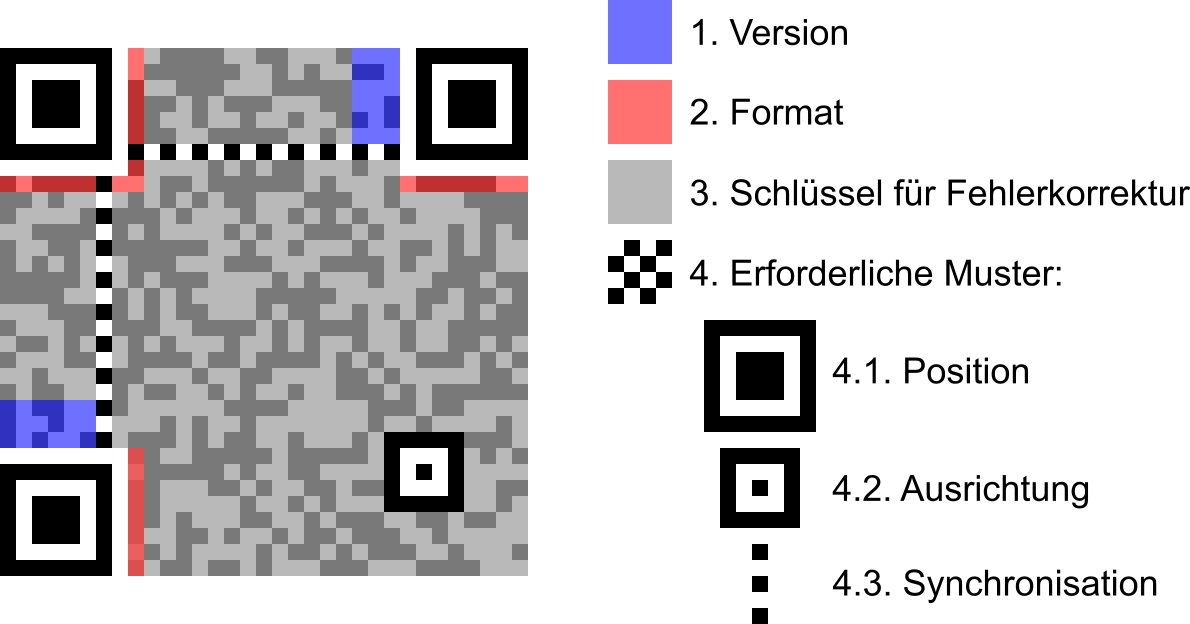
\includegraphics[scale=0.3]{images/QR_Code_Struktur_Beispiel.png}
\end{figure}
\todo{Quellen angeben!}

Des weiteren ist klar zu erkennen, dass der Code in drei von vier Ecken das Muster 4.1 vorweist. Diese dienen zur Bestimmung der Orientierung. Zusätzlich wird das Muster 4.2 (\emph{Finder Pattern}) verwendet um die Ausrichtung noch prezieser zu bestimmen. Bei größeren QR-Codes werden weitere Ausrichtungsmuster (Muster 4.2) eingefügt. Zwischen den \emph{Finder Patterns} befindet sich ein Streifen mit abwechselnd \glqq schwarz - weißen\grqq\  Punkten (\emph{Modulen}). Das sind die so genannten Synchronisations Muster oder auch \emph{Timming Patterns}.\\

Die Größe der QR-Codes ist beschränkt durch die Anzahl der \emph{Module}. Die Anzahl der \emph{Module} liegt zwischen $21 \times 21$ und $177 \times 177$. Beispielsweise sei der Code in Abbildung \ref{fig:struktur-qrcode} einer der Größe $21 \times 21$. Dann hätte ein \emph{Finder Pattern} die länge von $7$ \emph{Modules}. Die Anzahl ergibt sich aus der einzigartigen $1:1:3:1:1$ Struktur eines \emph{Finder Patterns}. Diese Fakten werden später ausschlagegebend sein bei der Rasterisierung des QR-Codes.

\section{Die verwendette Bibliothek OpenCV}
\emph{OpenCV}\footnote{WWW-Seite von dem Projekt \emph{OpenCV}: \url{http://opencv.org/}} ist eine Bibliothek mit Algorithmen spezialisiert auf \glqq Computer Vision\grqq . Sie wurde für die Programmiersprachen C/C++ geschrieben und steht unter BSD Lizenz. Es gibt mehrere Versionen der Bibliothek, die aktuellste ist die 3.2. Unser Programm setzt allerdings die Version 2.4, funktioniert aber auch mit neueren Version z.B \todo{Phill fragen}.



\chapter{Bildvorverarbeitung}
Die Bildvorverarbeitung ist ein essenzieller Schritt um die QR-Codes richtig lokalisieren zu können. Das Eingabebild soll in dieser Phase erstmal in ein Graustufenbild umgewandelt werden und danach binarisiert werden. \emph{OpenCV} bietet die Möglichkeit bilder direkt als Graustufenbild einzulesen oder sie in eins umzuwandeln. Das in Graustufen vorhandene Bild kann weiter verarbeitet werden.
Die Klasse \texttt{ImageBinarization} ist für die binarisierung zuständig. 
\inputCPP[label={lst:binarize}]{code/binarize-run.cpp}

Listing \ref{lst:binarize} zeigt den Ablauf der Binarisierung. In Zeile 4 wird die Methode \texttt{computeSmoothing} aufgerufen, die eine Gaußglättung auf dem Bild durchführt, um eventuelles Rauschen zu mindern. Im nächsten Schritt wird ein Farbstufen-Histogramm mithilfe der \texttt{computeHistogram} Methode berechnet. Um die best Mögliche Binarisierung zu erreichen, wurden drei Methoden zur Schwellwert Berechnung implementiert:
\begin{itemize}
	\item globales Schwellwertverfahren,
	\item Mittelwert basiertes Schwellwertverfahren,
	\item Gauß'sches Schwellwertverfahren.
\end{itemize} 
Im ersten durchlauf wird das globale Schwellwertverfahren angewandt. Sollte dies keine gültige Ergebnisse liefern (keine drei \emph{Finder Pattern} enthalten), so wird das nächste Verfahren gewählt. \\

Abhängig von der Wahl werden zwei verschiedene \emph{OpenCV} Methoden verwendett. Bei der globalen Schwellwert Berechnung wird auf die \texttt{threshold} Methode wie sie im Listing \ref{lst:globalthreshold} steht zurückgegriffen. Der Methode werden das Ein- und Ausgabe Bild, die Schwellwertgrenze, der maximale Farbwert und die Wahl des Algorithmus übergeben. 
\inputCPP[label={lst:globalthreshold}]{code/global-binarize.cpp}

Wir haben uns hier auf den Algorithmus von Otsu\footnote{Mehr Information zu dem Algorithmus auf der zugehörigen \emph{OpenCV} Seite:\url{http://docs.opencv.org/3.1.0/d7/d4d/tutorial_py_thresholding.html}} geeinigt, da er sehr gute Ergebnisse mit einer geringen Laufzeit liefert.\\

Bei den lokalen Schwellwertverfahren hingegen wird die Methode \texttt{adaptiveThreshold} verwendett. Listing \ref{lst:localthreshold} veranschaulicht die Methode die für die zwei lokalen Verfahren verwendet wird. Für die jeweiligen Verfahren wird der Parameter \texttt{adaptiveMethod} passend übergeben.
\inputCPP[label={lst:localthreshold}]{code/local-binarize.cpp}

Abbildung \todo{Abbildung} zeigt das Resultat.


\begin{figure}[h]
\center
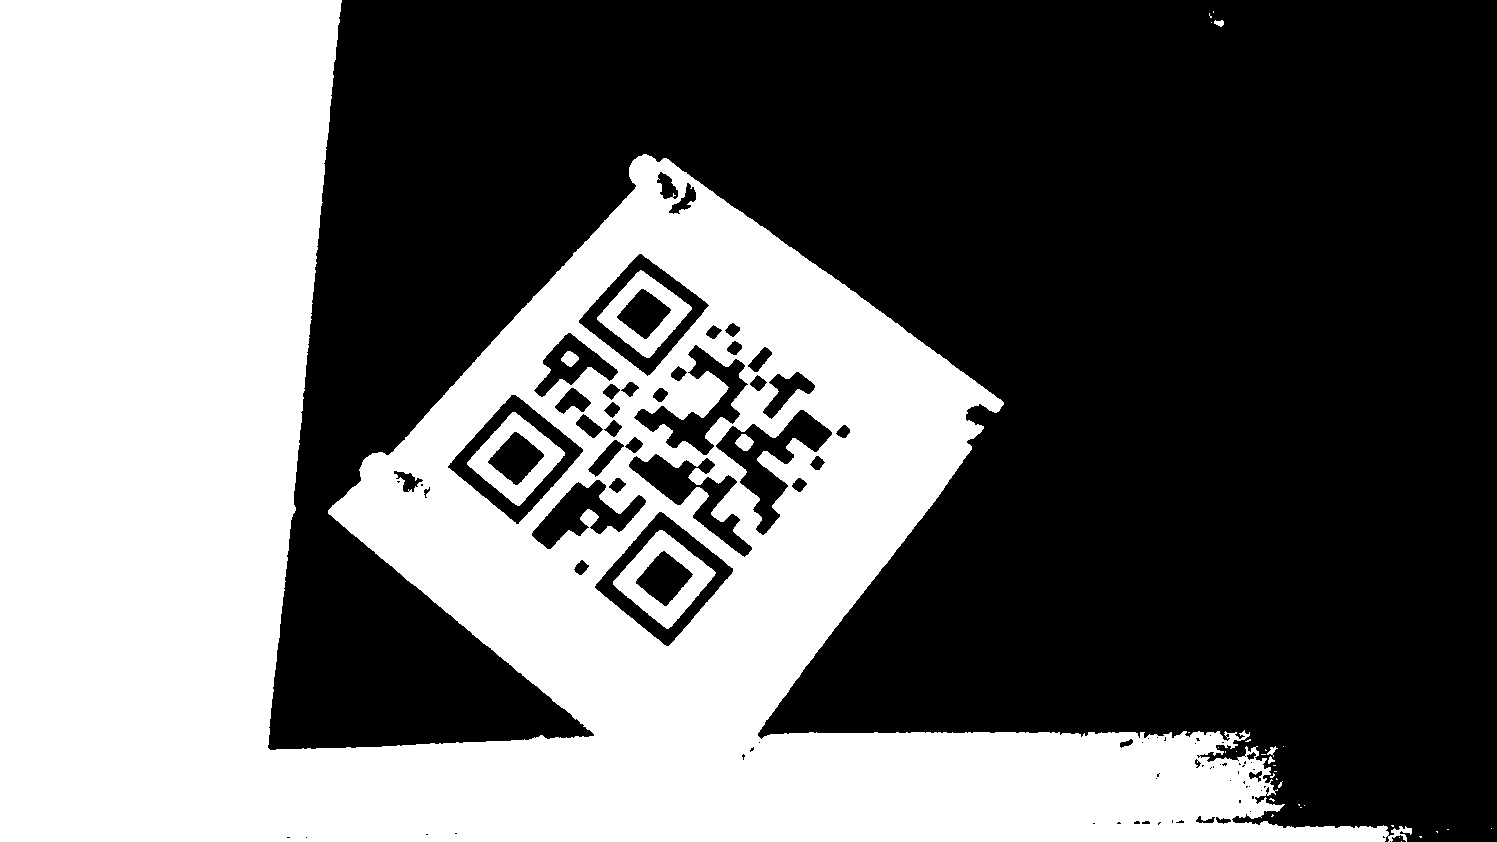
\includegraphics[scale=0.1]{images/qrcode-adler-wand_1___BINARIZED___.jpg}
\hspace{5px}
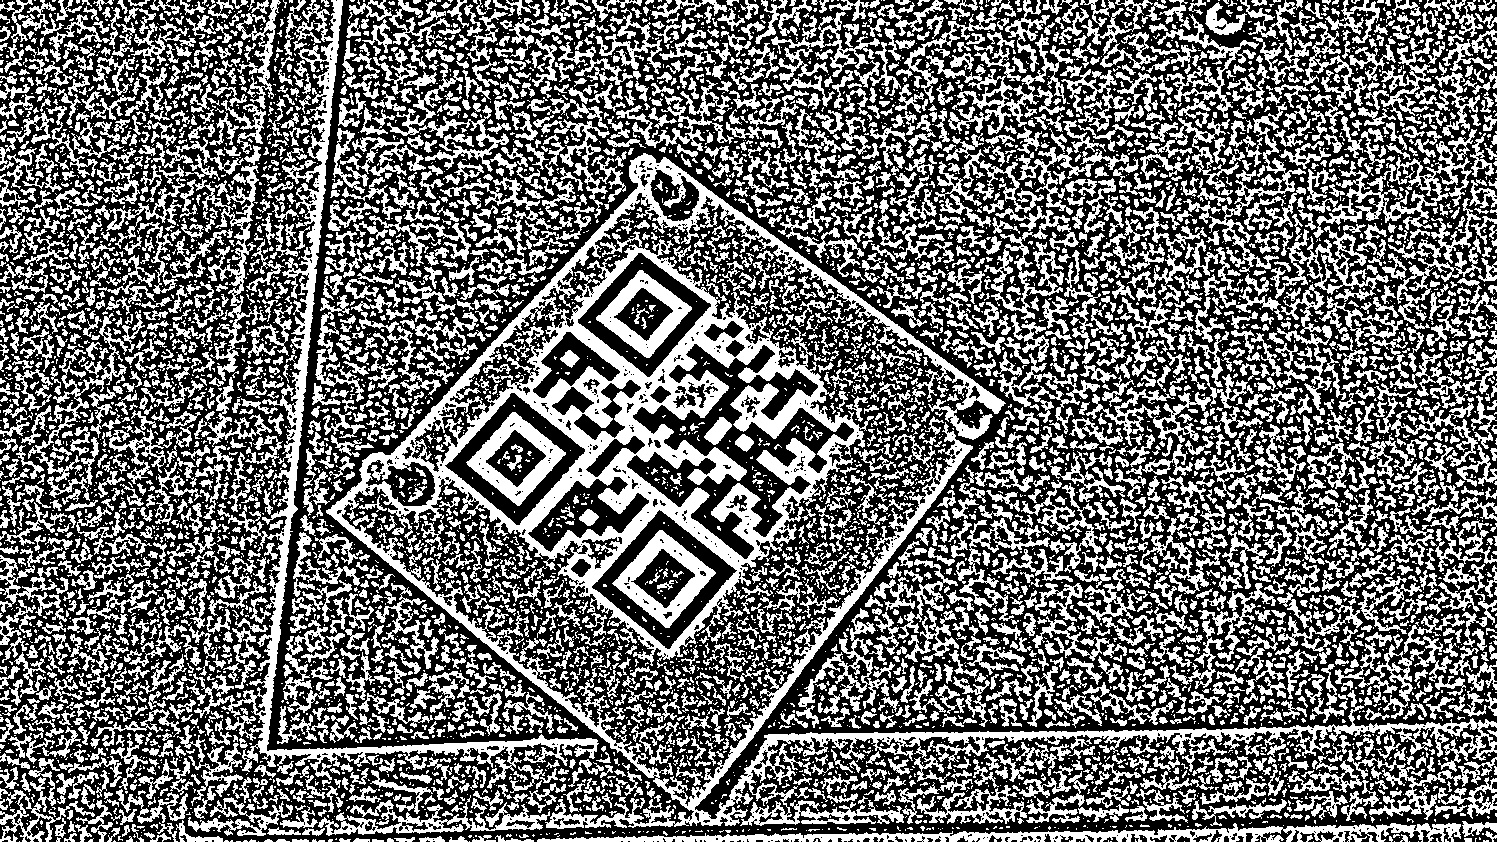
\includegraphics[scale=0.1]{images/qrcode-adler-wand_2___BINARIZED___.jpg}
\caption{Das Resultat der Binarisierung mit den jeweiligen Verfahren. Links global und Rechts lokal.}
\end{figure}

\chapter{Patternidentifikation}
